\documentclass{article}
\usepackage[utf8]{inputenc}
\usepackage[portuges]{babel}
\usepackage{csquotes}
\usepackage{geometry}
\usepackage[pdftex]{hyperref}
\usepackage{indentfirst}
\usepackage{amsthm}
\usepackage{amssymb}
\usepackage{amsmath}
\usepackage{xcolor}
\usepackage{tikz}
\usepackage{float}
\usepackage[backend = biber]{biblatex}
\addbibresource{referencias.bib}
\tikzstyle{format} = [rectangle, draw, fill = blue!20]
\usetikzlibrary{er,positioning}

\geometry{left = 3cm, top = 3cm, bottom = 2cm, right = 2cm}

\title{COVID-19 na Itália}
\author{Cristhian Grundmann \\
Igor Patrício Michels}
\date{2020.2}

\begin{document}

\maketitle

\section{Introdução}

O presente artigo visa descrever, por meio de um modelo epidemiológico de EDO's, os casos de COVID-19 na Itália. A modelagem se dará por meio de modelos de EDO's, os quais foram vistos durante as aulas de Modelagem de Fenômenos Biológicos (Modelagem Matemática IV) ministrada pelo professor Flávio Codeço Coelho da FGV - EMAp.

A situação italiana variou muito durante a pandemia, sendo o primeiro país europeu a atingir uma marca superior a 100 infectados pela COVID-19, fato que ocorreu após 25 dias do primeiro infectado, conforme análise dos gráficos do site Our World in Data \cite{owid}. Em parte, esses números se devem ao fato de que a Itália foi surpreendida com um paciente zero assintomático e um paciente um que custou a desenvolver sintomas, com este último tendo inúmeros compromissos na época em que foi infectado, no início de fevereiro \cite{dn}\cite{cm}.

Em março a situação continuou se agravando, principalmente na região da Lombardia, dessa forma, a partir de 09/03/2020, o governo italiano passou a tomar medidas severas de isolamento social \cite{piccolomini}. Já para os mortos em virtude da COVID-19, a Itália registrava, até 11 de março, um total de 827 mortes, sendo que os falecidos possuíam uma média de 81 anos, dos quais 88,7\% possuíam idade superior a 69 anos. Além disso, dois terços dos falecidos apresentavam quadro de diabetes, câncer, alguma doença cardiovascular ou fumavam. Os números continuaram subindo, sendo que no dia 15 de março os casos de COVID-19 na Itália já passavam de 22.000, com média de idade de 64 anos. Além disso, já haviam 1.625 mortes, a maior parte dessas por pessoas com mais de 69 anos \cite{REMUZZI20201225}\cite{10.1001/jama.2020.4344}.

Entre março e o final de abril as políticas governamentais de isolamento social atingem uma pontuação superior a 90 pontos no Índice de Rigor Governamental do Our World in Data \cite{owid}, o que se mostrou eficiente para diminuir o total de casos ativos \cite{italia}. Entre maio e meados de julho a quantidade de indivíduos atualmente positivados só decresceu, tendo uma certa estabilidade até meados de agosto, quando iniciou-se uma nova crescente nos casos ativos.

Apesar da nova crescente no número de casos, o número de mortos está muito abaixo da primeira onda de casos. Esse fato se dá, em especial, pela alta infecção de pessoas com idade inferior a 50 anos \cite{istoe_idade} em virtude da volta ao trabalho por parte da população \cite{folha_trabalho}. Além disso, a volta às aulas, de forma presencial, ocorreu no dia 14/09 \cite{uol_aulas}, o que está gerando um novo aumento no número de casos.

% \section{Revisão da Literatura}
% % trabalhos de modelagem sobre a situação da Itália

% Nessa seção iremos apresentar alguns dos trabalhos que buscaram modelar a epidemia de coronavírus na Itália. Estamos dando ênfase a modelos compartimentais, apresentando um modelo discreto e três modelos de EDO's.

% \subsection{Modelo SIRD discreto}
% 
Revisando a literatura, um dos primeiros trabalhos publicados foi o de Calafiore, Novara e Possieri, onde foi elaborado um modelo discreto com base no modelo SIR \cite{calafiore2020modified}. Nesse artigo os autores comentam que o trabalho foi feito de maneira rápida em virtude do contágio da COVID-19, tanto que a publicação se deu em 31 de março. A modelagem utilizou dados até 30 de março e buscou, com um modelo simples, analisar o contágio e a eficiência das medidas preventivas. Abaixo temos o modelo base do artigo
\begin{equation*}
    \begin{split}
        S(t + 1) & = S(t) - \beta \dfrac{S(t) I(t)}{S(t) + I(t)}, \\
        I(t + 1) & = I(t) + \beta \dfrac{S(t) I(t)}{S(t) + I(t)} - \gamma I(t) - \nu I(t), \\
        R(t + 1) & = R(t) + \gamma I(t), \\
        D(t + 1) & = D(t) + \nu I(t).
    \end{split}
\end{equation*}

Note que a ideia utilizada é um modelo SIR clássico discretizado, com as mortes em virtude de algo diferente da COVID-19 sendo ignoradas. Outra suposição do estudo foi o isolamento de cada região italiana\footnote{No estudo citado é feita a modelagem nacional e regional.}, a qual é aceitável em virtude das medidas de isolamento social que estavam em prática na época do estudo.

Para considerar os casos assintomáticos de COVID-19 os pesquisadores consideraram $I(t) = \alpha\tilde{I}(t)$, para algum $\alpha \geq 1$, o que gerou a seguinte alteração no modelo do estudo:
\begin{equation*}
    \begin{split}
        \tilde{S}(t + 1) & = \tilde{S}(t) - \beta \dfrac{\tilde{S}(t) \tilde{I}(t)}{\tilde{S}(t) + \tilde{I}(t)}, \\
        \tilde{I}(t + 1) & = \tilde{I}(t) + \beta \dfrac{\tilde{S}(t) I(t)}{\tilde{S}(t) + \tilde{I}(t)} - \gamma \tilde{I}(t) - \nu \tilde{I}(t), \\
        \tilde{R}(t + 1) & = \tilde{R}(t) + \gamma \tilde{I}(t), \\
        D(t + 1) & = D(t) + \alpha \nu \tilde{I}(t).
    \end{split}
\end{equation*}

Com essa alteração passa-se a considerar a transmissão do vírus por assintomáticos, resolvendo um dos problemas na modelagem dessa doença. Os resultados dessa modelagem foram interessantes. O modelo se ajustou muito bem aos dados que possuíam, entretanto o modelo subestimou a pandemia, tanto em tempo quanto em infecções. Pelo modelo, o pico de COVID-19 na Itália se daria no começo de abril, com uma quantidade de infectados entre 80 e 90 mil pessoas. Já na realidade o pico se deu na segunda metade de abril com quase 110 mil infectados. Note que o modelo fez uma aproximação razoavelmente boa, aproximando bem o pico da doença.
% 
% \subsection{Modelo SEPIAHQRD}

Outro modelo que surgiu nos estágios iniciais da pandemia, mas um pouco mais complicado foi o modelo SEPIAHQRD, proposto por Gatto et al. Eis o modelo SEPIAHQRD \cite{Gatto10484}:
\begin{figure}[H]
    \centering
    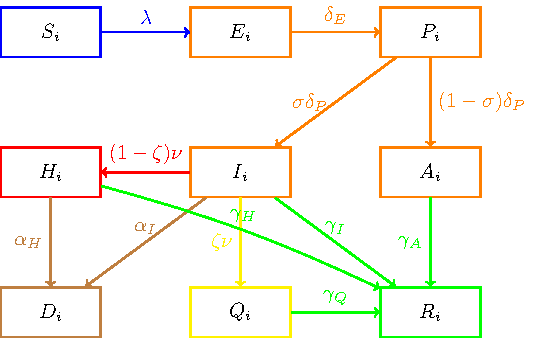
\includegraphics[page = 1]{Tikz - PDF/Tikz1.pdf}
\end{figure}

O que nos dá o seguinte conjunto de equações:
\begin{equation*}
    \begin{split}
        \dot{S} & = -\lambda S,\\
        \dot{E} & = \lambda S - \delta_E E, \\
        \dot{P} & = \delta_E E - \delta_P P, \\
        \dot{I} & = \sigma \delta_P P - (\eta + \gamma_I + \alpha_I) I, \\
        \dot{A} & = (1-\sigma) \delta_P P - \gamma_A A, \\
        \dot{H} & = (1-\zeta) \eta I - (\gamma_H + \alpha_H) H, \\
        \dot{Q} & = \zeta \eta I - \gamma_Q Q, \\
        \dot{R} & = \gamma_I I + \gamma_A A + \gamma_H H, \\
        \dot{D} & = \alpha_I I + \alpha_H H,
    \end{split}
\end{equation*}

\noindent onde $S$ representa os suscetíveis, $E$ os expostos, $P$ os pré-sintomáticos, $I$ os infectados, $A$ os assintomáticos, $H$ os hospitalizados, $Q$ os em quarentena, $R$ os recuperados e $D$ os mortos. Além disso, 
\[\lambda = \frac{\beta_P P + \beta_I I + \beta_A A}{S + E + P + I + A},\]

\noindent onde os parâmetros $\beta_P$, $\beta_I$ e $\beta_A$ ajustam a probabilidade de transmissão de cada classe transmissora. O trabalho ainda dividiu a população em 107 comunidades distintas e simulou a interação entre estas, além de considerar $\gamma_Q = \gamma_I = \gamma_H$ e $\gamma_A = 2\gamma_I$.

A estimação de parâmetros foi feita com estatística Bayesiana, usando o algoritmo Markov Chain Monte Carlo (MCMC) para computar a distribuição a posteriori.
% 
% \subsection{Modelo SIDARTHE}

Além do modelo SEPIAHQRD, outro modelo que surgiu nas fases inicias da pandemia explora o modelo SIDARTHE \cite{JOUR}. Tal modelo possui o seguinte desenho compartimental
\begin{figure}[H]
    \centering
    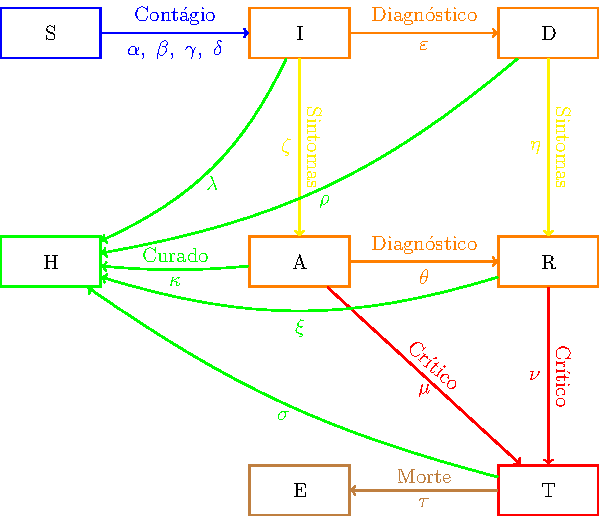
\includegraphics[page = 1]{Tikz - PDF/Tikz2.pdf}
\end{figure}

\noindent onde $S$ representa os suscetíveis, $I$ os assintomáticos não diagnosticados, $D$ os assintomáticos diagnosticados, $A$ os sintomáticos não diagnosticados, $R$ os sintomáticos diagnosticados, $T$ os indivíduos hospitalizados, $H$ os indivíduos curados e $E$ os que faleceram. Note que, assim como os modelos anteriores, as mortes que ocorrem por motivo distinto da COVID-19 são desprezadas. Tendo visto a ideia geral do modelo, vamos as equações propostas:
\begin{equation*}
    \begin{split}
        \dot{S}(t) & = -S(t)(\alpha I(t) + \beta D(t) + \gamma A(t) + \delta R(t)),\\
        \dot{I}(t) & = S(t)(\alpha I(t) + \beta D(t) + \gamma A(t) + \delta R(t)) - (\varepsilon + \zeta + \lambda)I(t), \\
        \dot{D}(t) & = \varepsilon I(t) - (\eta + \rho)D(t), \\
        \dot{A}(t) & = \zeta I(t) - (\theta + \mu + \kappa)A(t), \\
        \dot{R}(t) & = \eta D(t) + \theta A(t) - (\nu + \xi)R(t), \\
        \dot{T}(t) & = \mu A(t) + \nu R(t) - (\sigma + \tau)T(t), \\
        \dot{H}(t) & = \lambda I(t) + \rho D(t) + \kappa A(t) + \xi R(t) + \sigma T(t), \\
        \dot{E}(t) & = \tau T(t).
    \end{split}
\end{equation*}

Aqui $\alpha$, $\beta$, $\gamma$ e $\delta$ representam taxas de infecção, $\varepsilon$ e $\theta$ a probabilidade de detecção da doença, os parâmetros $\zeta$ e $\eta$ modelam a probabilidade de um infectado desenvolver sintomas, já $\mu$ e $\nu$ são parâmetros que denotam a probabilidade do desenvolvimento de sintomas que podem levar o indivíduo a óbito, o que foi modelado com o parâmetro $\tau$. Por fim, $\lambda$, $\rho$, $\kappa$, $\xi$ e $\sigma$ modelam a recuperação dos indivíduos.

Uma ideia muito interessante proposta no modelo SIDARTHE é a divisão do infectados em compartimentos separados, de acordo com seu status atual (assintomático/sintomático e diagnosticado/não diagnosticado). Essa divisão, juntamente com o estabelecimento de quatro parâmetros de infecção busca refletir a ideia de que pessoas infectadas mas que não sabem que portam o vírus tendem a ter uma taxa de transmissão diferente de pessoas que sabem que portam o vírus. Dessa forma, cada grupo de infectados irá transmitir a doença de acordo com um parâmetro diferente. Entre esses parâmetros, normalmente se tem $\alpha > \gamma$, uma vez que as pessoas tendem a evitar contato com pessoas que, mesmo sem diagnóstico de COVID-19, apresentam sintomas. Além dessa desigualdade, em geral vale também que $\gamma > \beta$ e $\gamma > \delta$, pois espera-se que indivíduos que estão cientes que portam o vírus fiquem em isolamento social.

Para efeito de modelagem, foi considerado $S + I + D + A + R + T + H + E = 1$, ou seja, foram tomadas tais medidas e divido o valor pela população italiana\footnote{Cerca de 60 milhões de pessoas.}. Com uma análise matemática, percebe-se que os equilíbrios desse modelo se dão apenas em estados em que temos $I = D = A = R = T = 0$, ou seja, quando o número de infetados zerar. Durante a modelagem, os autores variaram os parâmetros de acordo com decisões políticas adotadas no país, como a implementação de lockdown, por exemplo. Com essa modelagem, foi obtido um resultado interessante, com curvas similares as dos dados observados.
% 
% \subsection{Modelo fSEIRD}

O último modelo analisado foi o fSEIRD (forced SEIRD) com taxa de infecção sendo uma função do tempo com o objetivo de ajustar melhor os dados de acordo com as políticas de isolamento social tomadas pelo governo italiano \cite{piccolomini}.

Conforme o artigo já cita na introdução, o modelo foi bem ajustado aos dados quando tomados dados de três meses de epidemia. Já ao fazer uma análise dos primeiros estágios da epidemia, o modelo prevê os picos com diferença de poucos dias do pico real. Vale também ressaltar que o modelo foi aplicado em duas regiões italianas, Lombardia e Emília-Romanha, sendo de forma separada para cada região, uma vez que as medidas de isolamento social foram tomadas em períodos distintos em cada região.

Assim como os modelos SEPIAHQRD e SIDARTHE, esse modelo pode ser expresso por um sistema de EDO's:
\begin{equation}
    \label{piccolomini_model}
    \begin{split}
        \dfrac{dS}{dt} & = -\dfrac{\beta(t)}{N}SI, \\
        \dfrac{dE}{dt} & = \dfrac{\beta(t)}{N}SI - \alpha(t) E, \\
        \dfrac{dI}{dt} & = \alpha(t) E - \dfrac{1}{T_I}I, \\
        \dfrac{dR}{dt} & = \dfrac{1 - f(t)}{T_I}I, \\
        \dfrac{dD}{dt} & = \dfrac{f(t)}{T_I}I,
    \end{split}
\end{equation}

\noindent onde $N$ representa a população total, ou seja, $N = S + E + I + R + D$ e as demais letras latinas representam os compartimentos usuais do modelo SEIRD. Assim podemos ver que a população é constante, uma vez que a soma das derivadas acima é nula. Além disso, note que a taxa de infecção do vírus ($\beta(t)$), a taxa de incubação ($\alpha(t)$) e a fração dos indivíduos que morreram ($f(t)$) são funções do tempo. Por fim, $T_I$ representa o período infeccioso médio.

No modelo, Piccolomini e Zama dividem o tempo em $\rho$ intervalos $[t_k, t_{k + 1}], ~k = 0, \dots, \rho -1$ e, com isso, definem dois modelos fSEIRD: o fSEIRD$_r$ e o fSEIRD$_e$, ambos dependendo da escolha da função para $\beta$. Foram propostas as seguintes funções:
\[\beta_r(t) = \beta(t_k)\left(1 - \rho_k\dfrac{(t - t_k)}{t}\right), ~t \in (t_k, t_{k + 1}], ~\rho_k \in (0, 1)\]
\[\beta_e(t) = \beta(t_k)e^{- \rho_k(t - t_k)}, ~t \in (t_k, t_{k + 1}], ~\rho_k \geq 0,\]

\noindent para um valor inicial $\beta(t_0)$ atribuído. Já $\alpha(t)$ e $f(t)$ foram considerados constantes em cada intervalo de tempo, ou seja
\[\alpha(t) = \alpha_k, ~\alpha_k \geq 0, ~t \in (t_k, t_{k + 1}]\]
\[f(t) = f_k, ~f_k \in [0, 1], ~t \geq 0,\]

\noindent dessa forma, temos que o modelo definido em \ref{piccolomini_model} está bem definido. Além disso, vale que $R_0(t) = \beta(t)T_I$. Vale ressaltar que a ideia de tomar os parâmetros $\beta$, $\alpha$ e $f$ como uma função do tempo se deu em virtude das medidas de isolamento social implementadas, uma vez que ao tentar fitar os dados com parâmetros fixos não era obtido um resultado eficiente.

Para a calibração do modelo foram utilizadas algumas técnicas estatísticas como a BIC (Bayesian Information Criterion) para verificar qual partição do tempo seria a melhor possível, isto é, a que minimiza a BIC. No artigo, foi utilizada uma partição de $14$ dias para a modelagem na Lombardia e de $7$ dias na Emília-Romanha. Com tais parâmetros, o modelo foi fitado e conseguiu modelar muito bem os dados observados. Além disso, ao fitar o modelo apenas com os dados dos primeiros trinta dias de infecção na Itália o modelo também obteve um bom resultado, com o número de infectados estando bem próximo do número observado nos dados após os trinta primeiros dias de epidemia.

\section{Metodologia}
% Seção de Metodologia propondo um modelo matemático para a situação epidemiológica do país escolhido justificando a sua adequação para a situação epidemiológica observada até o momento no país. Esta seção deve descrever completamente o modelo e seus compartimentos, todas as suas equações acompanhadas de análise dimensional e descrição e interpretação de todos os parâmetros utilizados. Esta seção deverá ainda descrever o processo de captura dos dados epidemiológicos do país de interesse.

% \subsection{Escolha do Modelo}
% 
Após a revisão da literatura e análise de modelos, buscamos um modelo simples e que pudesse modelar de forma eficiente a epidemia. Dessa forma, modelos oriundos do SI foram descartados, uma vez que a reinfecção ocorre raramente \cite{again}. Outra família de modelos descartada foi a do modelo SIR, uma vez que, conforme vão ocorrendo as infecções, um grupo de pessoas expostas\footnote{Pessoas que portam o vírus mas ainda não transmitem o vírus.} vai se formando e, com isso, inclui-se no modelo um compartimento para expostos.

Com o passar do tempo, as pessoas passam a transmitir o vírus, assim as pessoas migram do compartimento E para o I. Por fim, a partir de I a pessoa irá se recuperar ou irá morrer, então entram os compartimentos R e D, formando, com isso, o modelo SEIRD.\footnote{Mais detalhes sobre cada compartimento serão vistos % na seção \ref{descrição_do_modelo}.}
mais adiante.}

Entretanto, conforme visto pela revisão da literatura, o modelo SEIRD nativo não conseguiu modelar de forma eficiente a situação italiana, assim, optamos por usar o modelo fSEIRD, ou forced SEIRD, o qual, conforme visto, é um modelo de EDO's adaptado do SEIRD, mas com que os parâmetros possam ser funções do tempo. Dessa forma, com os parâmetros sendo funções, temos a incorporação das decisões de autoridades à respeito do grau de isolamento social, o que possibilita um melhor ajuste aos dados, bem como auxilia no ajuste da nova onda de infecções que está ocorrendo na Itália, algo que não seria possível com o modelo SEIRD nativo.

% \subsection{Descrição do Modelo} \label{descrição_do_modelo}
% 
Nosso modelo trabalha de forma análoga aos demais modelos de EDO's, ou seja, de forma compartimental. Para a modelagem, optamos por trabalhar com os valores absolutos em cada compartimento e com população constante, dessa forma, a natalidade e a mortalidade natural foram desprezadas, o que implica em uma população constante\footnote{Nesse caso, população se refere ao número total de indivíduos, isto é, $S + E + I + R + D$.}, logo, sendo $N$ a população italiana, sempre vale que $N = S + E + I + R + D$. Abaixo temos o desenho compartimental do modelo.
\begin{figure}[H]
    \centering
    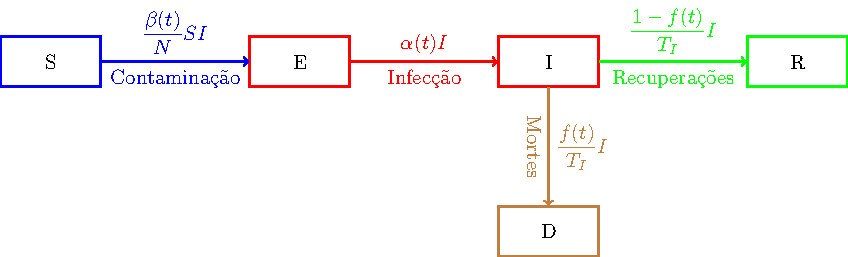
\includegraphics[page = 1]{Tikz - PDF/Tikz3.pdf}
\end{figure}

O qual nos dá o seguinte conjunto de equações:
\begin{equation}
    \label{fSEIRD}
    \begin{split}
        \dfrac{dS}{dt} & = -\dfrac{\beta(t)}{N}SI, \\
        \dfrac{dE}{dt} & = \dfrac{\beta(t)}{N}SI - \alpha(t) E, \\
        \dfrac{dI}{dt} & = \alpha(t) E - \dfrac{1}{T_I}I, \\
        \dfrac{dR}{dt} & = \dfrac{1 - f(t)}{T_I}I, \\
        \dfrac{dD}{dt} & = \dfrac{f(t)}{T_I}I.
    \end{split}
\end{equation}

Como possuímos os dados liberados diariamente pelo \textit{Our World in Data} \cite{owid}, estamos considerando o tempo em dias. Mas note que essas equações ainda não definem completamente o modelo, uma vez que nem todos os parâmetros são constantes. Para finalizar a definição do modelo, dividimos o tempo em $\rho$ intervalos $[t_k, t_{k + 1}], ~k = 0, \dots, \rho -1$, dado que as medidas públicas na Itália foram variando conforme o tempo. Além disso, é interessante tomar uma taxa de infecção decrescente, uma vez que decretos e medidas de isolamento social não são totalmente aplicadas assim que ocorre a publicação da ordem. Assim, definimos
\[\beta_r(t) = \beta(t_k)\left(1 - \rho_k\dfrac{(t - t_k)}{t}\right), ~t \in (t_k, t_{k + 1}], ~\rho_k \in (0, 1)\]
\[\beta_e(t) = \beta(t_k)e^{- \rho_k(t - t_k)}, ~t \in (t_k, t_{k + 1}], ~\rho_k \geq 0,\]

\noindent para um valor inicial $\beta(t_0)$ atribuído. Já $\alpha(t)$ e $f(t)$ serão considerados constantes em cada intervalo de tempo, ou seja
\[\alpha(t) = \alpha_k, ~\alpha_k \geq 0, ~t \in (t_k, t_{k + 1}]\]
\[f(t) = f_k, ~f_k \in [0, 1], ~t \in (t_k, t_{k + 1}].\]

Agora, tendo todas as equações definidas, iremos para a descrição de cada compartimento utilizado.

\subsection{Compartimento S}

O primeiro compartimento do modelo é o S, representando a classe das pessoas suscetíveis, isto é, que não estão contaminadas mas que podem contraí-la.

Uma vez que um indivíduo contrai a doença, ele muda da classe S para a classe E, e nunca mais volta a ser suscetível. Isso significa que ou ele morre pela doença ou ele se recupera e se torna imune. A variação desse compartimento se dá por
\[\dfrac{dS}{dt} = -\dfrac{\beta(t)}{N}SI.\]

Essa equação modela a contaminação da doença fazendo com que os indivíduos contaminados saiam da classe S conforme a lei da ação das massas, ou seja, a quantidade de novos infectados é proporcional ao produto do número de indivíduos suscetíveis com o número de indivíduos infectados. Note que essa proporção é dada pelo parâmetro $\beta(t)$, medido em $dias^{-1}$.\footnote{Uma análise mais detalhada da dimensão de $\beta(t)$, bem como das demais variáveis, será vista % na seção \ref{analise_dimensional}.}
mais adiante.} A variável I representa o compartimento dos indivíduos infecciosos, e N é a população total do sistema.

\subsection{Compartimento E}

Quando um indivíduo S é contaminado por algum I, ele migra para a classe E, que representa a classe dos indivíduos expostos, isto é, que estão com a doença, mas não a transmitem. Sua variação se dá por
\[\dfrac{dE}{dt} = \dfrac{\beta(t)}{N}SI - \alpha(t) E,\]

\noindent ou seja, essa classe recebe os indivíduos que a classe S perde por contaminação e perde os indivíduos contaminados que passam a transmitir. Essa perda é proporcional ao tamanho da classe, e ajustado pelo parâmetro $\alpha(t)$, medido em $dias^{-1}$.

\subsection{Compartimento I}

A variável I representa a classe dos infecciosos, ou seja, os indivíduos que estão contaminados e que contamina os suscetíveis. Sua variação se dá pela equação
\[\dfrac{dI}{dt} = \alpha(t) E - \dfrac{1}{T_I}I.\]

Essa classe recebe os indivíduos que passam a ser transmissores e perde para duas classes. Uma delas é a de recuperados, enquanto a outra é a de mortos (pela doença apenas). É claro que as proporções entre essas perdas não são iguais. No modelo, a taxa combinada é $1/T_I$, onde $T_I$ representa o período médio de infecção, em dias.

\subsection{Compartimento R}

A classe R representa os indivíduos que contraíram a doença e se recuperaram dela, ou seja, indivíduos que não transmitem mais e são imunes a ela. A classe só recebe indivíduos da classe I, sem perder nenhum indivíduo. Seu acréscimo se dá pela equação
\[\dfrac{dR}{dt} = \dfrac{(1 - f(t))}{T_I}I.\]

Como a taxa total de saída da classe I é $1/T_I$, o parâmetro $f(t)$ é a proporção de indivíduos que morre da taxa total $1/T_I$. Por isso que a taxa de saída dessa classe é o complementar $\frac{1 - f(t)}{T_I}$. Esse parâmetro pode depender do tempo, assim como $\beta(t)$ e $\alpha(t)$, mas é adimensional.

\subsection{Compartimento D}

A classe D representa os indivíduos que morreram pela doença. Assim como a classe R, a classe D só recebe indivíduos da classe I, e não perde nenhum indivíduo. Dessa forma, seu acréscimo é dado por
\[\dfrac{dD}{dt} = \dfrac{f(t)}{T_I}I.\]

Como já definido anteriormente, $f(t)$ é a proporção dos indivíduos que morrem da em relação a taxa total, que é $\frac{1}{T_I}$. 

\subsection{Demais Parâmetros}

Os demais termos do sistema de EDO's ($N$, $\alpha(t)$, $\beta(t)$ e $f(t)$) são parâmetros gerais do modelo. Como já definido anteriormente, $N$ é a população total do sistema, ou seja, $N = S + E + I + R + D$. Já $\beta(t)$ é um parâmetro funcional que denota a taxa de transmissão do vírus, $\alpha(t)$ denota a taxa com que os indivíduos se tornam infecciosos e, finalmente, $f(t)$ representa a fração da população que acaba falecendo em virtude da COVID-19.

% \subsection{Análise Dimensional} \label{analise_dimensional}
% 
Como estamos trabalhando com populações, sabemos que $[N] = [S] = [E] = [I] = [R] = [D] = [\text{pessoas}]$. Dessa forma, como comentado % na seção \ref{descrição_do_modelo}
anteriormente, temos que o tempo é medido em dias, assim, vale que $[T_I] = [\text{dias}]$
\[\left[\dfrac{dS}{dt}\right] = \left[\dfrac{dE}{dt}\right] = \left[\dfrac{dI}{dt}\right] = \left[\dfrac{dR}{dt}\right] = \left[\dfrac{dD}{dt}\right] = \dfrac{\text{pessoas}}{\text{dias}}.\]

Dessa forma, temos
\begin{equation*}
    \begin{split}
        \dfrac{dS}{dt} & = -\dfrac{\beta(t)}{N}SI \\
        \left[\dfrac{\text{pessoas}}{\text{dias}}\right] & = \dfrac{[\beta(t)]}{[N]}[S][I] \\
        \dfrac{[\text{pessoas}]}{[\text{dias}]} & = \dfrac{[\beta(t)]}{[\text{pessoas}]}[\text{pessoas}][\text{pessoas}] \\
        \dfrac{1}{[\text{dias}]} & = [\beta(t)]
    \end{split}
\end{equation*}

Além disso, temos
\begin{equation*}
    \begin{split}
        \dfrac{dE}{dt} & = \dfrac{\beta(t)}{N}SI - \alpha(t) E \\
        \left[\dfrac{\text{pessoas}}{\text{dias}}\right] & = \dfrac{[\beta(t)]}{[N]}[S][I] - [\alpha(t)][E] \\
        \dfrac{[\text{pessoas}]}{[\text{dias}]} & = [\text{dias}^{-1}][\text{pessoas}] - [\alpha(t)][\text{pessoas}]
    \end{split}
\end{equation*}

\noindent mas sabemos que, como a expressão da direita acima é uma subtração, vale que a unidade dimensional dos dois termos deve ser igual, ou seja, $[\alpha(t)] = [\text{dias}^{-1}]$. Por fim, faremos a análise dimensional de $f(t)$:
\begin{equation*}
    \begin{split}
        \dfrac{dD}{dt} & = \dfrac{f(t)}{T_I}I \\
        \left[\dfrac{\text{pessoas}}{\text{dias}}\right] & = \dfrac{[f(t)]}{[T_I]}[I] \\
        \dfrac{[\text{pessoas}]}{[\text{dias}]} & = \dfrac{[f(t)]}{[\text{dias}]}[\text{pessoas}]
    \end{split}
\end{equation*}

\noindent de onde conclui-se que $f(t)$ é adimensional.

% \subsection{Obtenção dos Dados}
% 
Todos os dados utilizados para realizar a modelagem foram obtidos exclusivamente do Our world in data \cite{owid}, através de sua página voltada a epidemia de COVID-19. Para trabalhar com os mesmos, baixamos o arquivo csv com os dados necessários e manipulamos os mesmos com o SageMath 9.0. Todos os arquivos estarão disponíveis no GitHub do artigo \cite{github}.

\printbibliography

\end{document}